\documentclass[conference]{IEEEtran}
\IEEEoverridecommandlockouts
% The preceding line is only needed to identify funding in the first footnote. If that is unneeded, please comment it out.
\usepackage{cite}
\usepackage{amsmath,amssymb,amsfonts}
\usepackage{algorithmic}
\usepackage{graphicx}
\usepackage{textcomp}
\usepackage{xcolor}
\usepackage{listings}
\lstset{
  basicstyle=\ttfamily,
  columns=fullflexible,
  frame=single,
  language=Python,
  breaklines=true,
%  postbreak=\mbox{\textcolor{red}{$\hookrightarrow$}\space},
}
\def\BibTeX{{\rm B\kern-.05em{\sc i\kern-.025em b}\kern-.08em
    T\kern-.1667em\lower.7ex\hbox{E}\kern-.125emX}}
\begin{document}

\title{Project 11: Semantic Analysis}

\author{\IEEEauthorblockN{Dennis Neumann}
\IEEEauthorblockA{Oulu, Finland\\
dennis2.neumann@student.uni-siegen.de}
\and
\IEEEauthorblockN{Muhammad Sheraz Khan}
\IEEEauthorblockA{City, Pakistan\\
Sherazkhan1234@gmail.com}
}

\maketitle

\begin{abstract}
Semantic similarity has been used for multiple tasks regarding natural language processing for many years now. Various static and lexica-based methods for analyzing semantic similarity such as Wu-Palmer and Leacock-Chodorow with different approaches and results exist to determine the similarity between given phrases. This project aims to show how the dynamic and web-based similarity methods of the WebJaccard similarity work in comparison to the static methods with the help of the Python Natural Language Toolkit and google search.
\end{abstract}

\begin{IEEEkeywords}
semantic similarity, natural language processing, language processing, semantic, analysis, google search
\end{IEEEkeywords}

\section{Introduction}

In contrast to static semantic similarity analysis methods which are based on lexical search using WordNet, Wikipedia and text corpora \cite{radinsky}, the WebJaccard similarity (WebSim) introduces a more dynamic way to determine the relation of words, since those can change the meanings over time, \cite{websim} for example the word \textit{Tesla} nowadays can not only be associated with Nikola Tesla but also with the electric car brand of the same name. \\All methods have their own approaches to calculate the similarities which can be overwhelming for those not knowing how well they perform on the same set of words. For a good comparison between the static approaches with the dynamic methods, the WebSim will include the page-count-based similarity as well as the procentual overlap similarity.\\

Chapter~\ref{sec:methodology} introduces to the tasks for this project, the used tools and libraries and how the results wil be saved and visualized. Chapter~\ref{sec:implementation} shows the implementation details. In chapter~\ref{sec:results} the achieved results are shown and discussed.  Chapter~\ref{sec:results} concludes this project documentation and sums up the content.

\section{Methodology}\label{sec:methodology}

\subsection{Tasks}


\subsection{synsets}
According to the requirements for this project, the similarity methods have to be applied on at least ten synonym set ("synset") pairs \textit{(P,Q)}. . The pairs should include the three cases, in which a) \textit{P} is a synonym of \textit{Q}, b) \textit{P} is an antonym of \textit{Q}, c) \textit{P} has an entailment relation to \textit{Q}. For the tasks of this project, following synset pairs were selected:
\begin{itemize}
\item pleased - excited
\item run - rush
\item displeased - upset
\item sleep - nap
\item laugh - weep
\item rich - poor
\item drunk - sober
\item mobile phones - cell phones
\item introvert - extrovert
\item huawei - iphone
\item run - sweat
\item contested - won
\item fell - broken
\end{itemize}
Many synsets are not applicable to use together in some of the similarity methods, since they are not sharing common hypernyms \cite{perkins}. Therefore, the choice of synset pairs is very important for applying and testing them against all similarities. This issue is discussed further in chapter~\ref{subsec:wup}.

\subsection{Tools and Libraries}
In this project, following tools and packages were used for corresponding purposes:
\begin{itemize}
\item NLTK : ...
\end{itemize}

\section{Implementation}\label{sec:implementation}

\subsection{Preliminary Work}
For the purposes of understanding and for avoiding recurring code segments, this short chapter shows code segments related to the implementations in the following chapters.

\subsubsection{Visualization of Synsets and Results}
To visualize the similarity results for the synsets defined in~\ref{sec:methodology}, the synset pairs will be saved to the table \textit{pair\_words\_df} via the \textit{DataFrame} Python class. For every similarity, 

\begin{lstlisting}[frame=single, label=lst:table, caption={}, captionpos=b]]
sim_layer = [['pleased', 'Excited'], ['run', 'rush'], ...]
...
pair_words_df = pd.DataFrame(sim_layer, columns=['P', 'Q'])
pair_words_df['Column name'] = ''

for i in range(len(synsets)):
    pair_words_df.iloc[i,k] = ...
\end{lstlisting}

\subsubsection{Pre-Processing function}\label{sec:preproc}
In case of synsets of word length>1,  pre-processing should be performed. It has to contain the conversion in lower case, removal of special characters and lemmatizer for removing words with only one character as well as stopwords. The code segment~\ref{lst:preproc} demonstrates the important steps taken for the pre-processing with the help of the Regular expression operations package \textbf{re}.

\begin{lstlisting}[frame=single, label=lst:preproc, caption={Pre-processing for synsets of word length>1}, captionpos=b]]
def pre_processing(text):

    text = text.split(' ')
    text = [word.strip().lower() for word in text if word.lower() not in stopwords]
    rx = re.compile('([&#.:?!-()])*')
    text = [rx.sub('', word) for word in text]
    
# selecting only the alpha bets and words length greater than 1
    text = [word for word in text if len(word)>1 and word.isalpha()]
#     if some word appear more than 1, remove others
    unique = set(text)
    unique = [lemmatizer.lemmatize(word) for word in unique]
    
# storing after processing in third column
    return ' '.join(text)
\end{lstlisting}

\subsection{WebJaccard page count similarity}\label{subsec:webjac}
The first task consisted of implementing the WebJaccard similarity based on page count and calculate the similarity coefficient. Where \textit{H(P)} in \ref{fig:pagecount} are the results of the pair key P and \textit{H(Q)} the results of pair key Q, \textit{H(PQ)} are the results when searching for P and Q together. This similarity coefficient  is calculated as followed:
\begin{figure}[h]\label{fig:pagecount}
\centerline{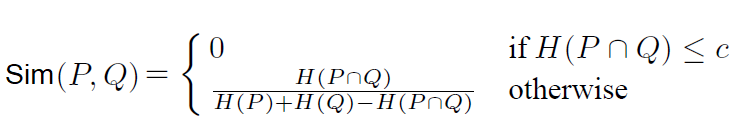
\includegraphics[scale=0.6]{img/pagecount.png}}
\caption{Formula for page-count-based WebJaccard similarity \cite{websim}.}
\label{fig}
\end{figure}

For the implementation we used the Google Search API. To use the \textit{search} function properly, some parameters have to be considered as seen in~\ref{lst:googlesearch}: whereas \textit{num} is the number of results and the maximum number is 10, the maximum request number per day is 100. The \textit{pause} between every requests also needs to be adjusted as a too high amount might slow down the process too much and a too low number might end up in an IP block by Google \cite{search}.

\begin{lstlisting}[frame=single, label=lst:googlesearch, caption={Google search function}, captionpos=b]
def google_search(query):
    return search(query, lang = 'en', num = 10, start = 0, stop = None, pause = 2.0)
\end{lstlisting}

Now the function can be used to get the results for each pair (P,Q). To get the page count, the \textit{len()} function is used on the returned \textit{list} of results (see~\ref{lst:hpq}). Once each \textit{H(P)}, \textit{H(Q)} and \textit{H(PQ)} results are saved in according variables \textit{count\_p}, \textit{count\_q} and \textit{count\_pq}, they can be used to calculate the Jaccard similarity coefficient. The \textit{threshold} is used to determine the minimum number of results. If the number of results is less than the threshold, the coefficient is 0 \cite{websim}. For the chosen synset pairs, there is no need for pre-processing the input since they only contain one word. Since the google API has a limitation of searching for one pair per hour, the values of the WebJaccard similarity had to be calculated one after another. To save the time, the calculated values were saved inthe array \textit{web\_results}.

\begin{lstlisting}[frame=single, label=lst:hpq, caption={Getting google results and calculation of WebJaccard similarity}, captionpos=b]]
def sim(P, Q, threshold, pre_process=False):
    if pre_process:
        P = pre_processing(P)
        Q = pre_processing(Q)

    results_p = google_search(P)
    count_p = len(list(results_p))

    results_q = google_search(Q)
    count_q = len(list(results_q))
    
    results_pq = google_search('{} AND {}'.format(P,Q))
    count_pq = len(list(results_pq))
    
    if count_pq <= threshold:
        return 0
    
    else:
        return (count_pq) /(count_p + count_q - count_pq)
...
web_results = [0.700, 0.960, 0.564, ...]
\end{lstlisting}

\subsection{Wu-Palmer-, Path- and Leacock-Chodorow-Similarity}\label{subsec:wup}
Unlike the WebJaccard similarity which has to be implemented manually, the WordNet Python library has predefined functions for the WuPalmer-Similarity (WUP) as well as the Path-Similarity (PATH) and Leacock-Chodorow-Similarity (LCH). The code segment~\ref{lst:wup} demonstrates the use of the \textit{wup\_similarity()}, \textit{path\_similarity()} and \textit{lch\_similarity()} functions on the self defined synsets from~\ref{sec:methodology}. The only pre-processing which has to be taken care of is to convert all synset's characters to lower case.

\begin{lstlisting}[frame=single, label=lst:wup, caption={Use of WUP, PATH and LCH}, captionpos=b]
def wordnet_sim(P, Q):
    P=wordnet.synsets(P.lower())
    Q=wordnet.synsets(Q.lower())

    for i in range(len(P)):
        for k in range(len(Q)):
...
            chod_sim = P[i].lch_similarity(Q[k])
            wup.append(P[i].wup_similarity(Q[k]))
            path.append(P[i].path_similarity(Q[k]))
\end{lstlisting}

\subsection{Snippet Similarity}\label{subsec:wup}

Besides the pagecount based similarity, the WebSim also includes a websearch snippet based similarity (SnippetSim) which is calculated as followed:

(TODO)

Where x is the number of common words, y is the number of combined unique words.

To achieve it, Google's Custom Search JSON API was used to retrieve the search results \cite{customsearch}. First an API key has to be created \cite{customsearch} and a Custom Engine ID (\textit{cx}) generated. These have to be inserted in the corresponding \textit{build()} function to make the source code work. The implementation is shown in the following code segment~ref{lst:snippetsim}:

\begin{lstlisting}[frame=single, label=lst:snippetsim, caption={Connection to Google Search API}, captionpos=b]
def google_snippets(query, num=10):
    query_service = build(serviceName="customsearch", version="v1", developerKey='...') 
    query_results = query_service.cse().list(q=query,cx='...', num=num).execute()
     return query_results['items']
\end{lstlisting}

For this similarity, the preprocessing function~\ref{lst:preproc} from chapter~\ref{sec:preproc} has to be used. For the calculation of the SnippetSim in this project, the first 5 results were taken. Based on the formula shown in (TODO) the implementation of the SnippetSim looks roughly as followed in~\ref{lst:snippetsim}):

\begin{lstlisting}[frame=single, label=lst:snippetsim, caption={Connection to Google Search API}, captionpos=b]
def sim_snippets(snipp_p, snipp_q):
  for i in range(5):
        snippets_p += pre_processing(snippet_p)     
        snippets_q += pre_processing(snippet_p)
    
    common_words = len(set(snippets_p.strip().split(' ')) & set(snippets_q.strip().split(' '))) 
    combined_unique_words = len(set(snippets_p + snippets_q))
    
  return common_words/combined_unique_words
\end{lstlisting}

\section{Results and discussions}\label{sec:results}

WebSim and SnippetSim also work on buzzwords like "Huawei - iPhone" and "Trump - Biden", while WordNet are not able to do that.

As mentioned in chapter~\ref{sec:methodology}, many pair words exist in which the combination of such do not work together, which causes some of the methods showing the similarity results as "None" \cite{perkins}, or in the case of LCH the pairs cause a compilation error "Computing the lch similarity requires synset1 and synset2 to have the same part of speech" \cite{wordnet}. So one of the challenges with the tasks in chapter~\ref{subsec:wup} and \ref{subsec:webjac}


\section{Conclusion}\label{sec:conclusion}

In this project the 



\bibliography{bibtex} 
\bibliographystyle{ieeetran}

\end{document}
